%% Manual for grid generator

\documentclass[12pt, a4paper]{article}
\usepackage[nofoot]{geometry}
\usepackage{graphicx}
\usepackage{fancyhdr}
\usepackage{amsfonts}
\usepackage[center]{subfigure}

%% Modify margins
\addtolength{\oddsidemargin}{-.25in}
\addtolength{\evensidemargin}{-.25in}
\addtolength{\textwidth}{0.5in}
\addtolength{\textheight}{0.25in}
%% SET HEADERS AND FOOTERS

\pagestyle{fancy}
\fancyfoot{}
\renewcommand{\sectionmark}[1]{         % Lower case Section marker style
  \markright{\thesection.\ #1}}
\fancyhead[LE,RO]{\bfseries\thepage}    % Page number (boldface) in left on even
                                        % pages and right on odd pages 
\renewcommand{\headrulewidth}{0.3pt}

\newcommand{\code}[1]{\texttt{#1}}
\newcommand{\file}[1]{\texttt{\bf #1}}

%% commands for boxes with important notes
\newlength{\notewidth}
\addtolength{\notewidth}{\textwidth}
\addtolength{\notewidth}{-3.\parindent}
\newcommand{\note}[1]{
\fbox{
\begin{minipage}{\notewidth}
{\bf NOTE}: #1
\end{minipage}
}}

\newcommand{\pow}{\ensuremath{\wedge} }
\newcommand{\poweq}{\ensuremath{\wedge =} }

\newcommand{\dd}[2]{\ensuremath{\frac{d #1}{d #2}}}
\newcommand{\ddd}[2]{\ensuremath{\frac{d^2 #1}{d #2^2}}}
\newcommand{\deriv}[2]{\ensuremath{\frac{\partial #1}{\partial #2}}}
\newcommand{\dderiv}[2]{\ensuremath{\frac{\partial^2 #1}{\partial {#2}^2}}}
\newcommand{\Vpar}{\ensuremath{V_{||}}}
\newcommand{\Gradpar}{\ensuremath{\partial_{||}}}
\newcommand{\Divpar}{\ensuremath{\nabla_{||}}}
\newcommand{\DivXgradX}[2]{\ensuremath{\nabla_\psi\left(#1\partial_\psi #2\right)}}
\newcommand{\DivParGradPar}[2]{\ensuremath{\nabla_{||}\left(#1\partial_{||} #2\right)}}

\newcommand{\apar}{\ensuremath{A_{||}}}
\newcommand{\hthe}{\ensuremath{h_\theta}}
\newcommand{\Bp}{\ensuremath{B_\theta}}
\newcommand{\Bt}{\ensuremath{B_\zeta}}

\newcommand{\Vec}[1]{\ensuremath{\mathbf{#1}}}
\newcommand{\bvec}{\Vec{b}}
\newcommand{\kvec}{\Vec{\kappa}}
\newcommand{\vvec}{\Vec{v}}
\newcommand{\bxk}{\bvec_0\times\kvec_0\cdot\nabla}
\newcommand{\Bvec}{\Vec{B}}
\newcommand{\Bbar}{\overline{B}}
\newcommand{\Lbar}{\overline{L}}
\newcommand{\Tbar}{\overline{T}}
\newcommand{\Jvec}{\Vec{J}}
\newcommand{\Jpar}{J_{||}}
\newcommand{\delp}{\nabla_\perp^2}
\newcommand{\Div}[1]{\ensuremath{\nabla\cdot #1 }}
\newcommand{\Curl}[1]{\ensuremath{\nabla\times #1 }}
\newcommand{\rbp}{\ensuremath{R\Bp}}
\newcommand{\rbpsq}{\ensuremath{\left(\rbp\right)^2}}
\newcommand{\Rvec}{\ensuremath{\hat{\Vec{R}}}}
\newcommand{\Zvec}{\ensuremath{\hat{\Vec{Z}}}}
\newcommand{\phivec}{\ensuremath{\hat{\Vec{\phi}}}}
\newcommand{\ehat}{\ensuremath{\hat{\Vec{e}}}}
\newcommand{\sbp}{\ensuremath{\sigma_{B\theta}}}

\begin{document}
\title{Tokamak grid generator in IDL}
\author{B.D.Dudson\dag, M.V.Umansky\S \\
\dag Department of Physics, University of York, York YO10 5DD, UK \\
\S Lawrence Livermore National Laboratory, CA 94550, USA\\

\includegraphics[width=0.2\paperwidth, keepaspectratio]{hypnotoad.png}}

\maketitle

\tableofcontents

\section{Introduction}

Generation of field-aligned grids is non-trivial for edge tokamak simulations
due to magnetic x-points and material surfaces. This grid generator has 
the following features:
\begin{itemize}
  \item Written entirely in IDL. Although some might call this a bug, it does mean that nothing needs to be compiled, and (in theory) this code should work everywhere that IDL is installed.
  \item Automatically adjusts settings when needed. The grid produced can 
    be customised, but the minimum number of inputs is very small
    (number of grid points and a psi range). The psi range asked for is
    adjusted to fit within the boundary.
  \item Can handle an arbitrary number of x-points. Whilst not of obvious
    benefit since tokamak equilibria are at most double-null, this means the
    code is quite generalised and can cope with ``strange'' configurations.
    Hopefully this will help make the code more resilient.
\end{itemize}

For a more complicated grid generator which can produce grids conforming
to boundaries, see the CARRE grid generator\footnote{``CARRE: a
quasi-orthogonal mesh generator for 2D edge plasma modelling'' by R. Marchand
and M. Dumberry. Comp. Phys. Comm. 96 (1996) pp 232-246} which produces
input files for B2, or UEDGE\footnote{Rognlien et al 1992 J. Nucl. Mater. 196–198 347} which can also be used to produce input to BOUT/BOUT++.

\section{Using the Hypnotoad}

The easiest way to generate grids is using the GUI called ``Hypnotoad''
(yes, it is named after the creature from Futurama, for no particularly good reason). Start IDL then run:
\begin{verbatim}
IDL> hypnotoad
\end{verbatim}
This should produce a window which looks like Figure~\ref{fig:screen_0}.
The appearance will vary between operating systems, and the screenshots
are from IDL running on Linux.
\begin{figure}[hp!]
  \centering
  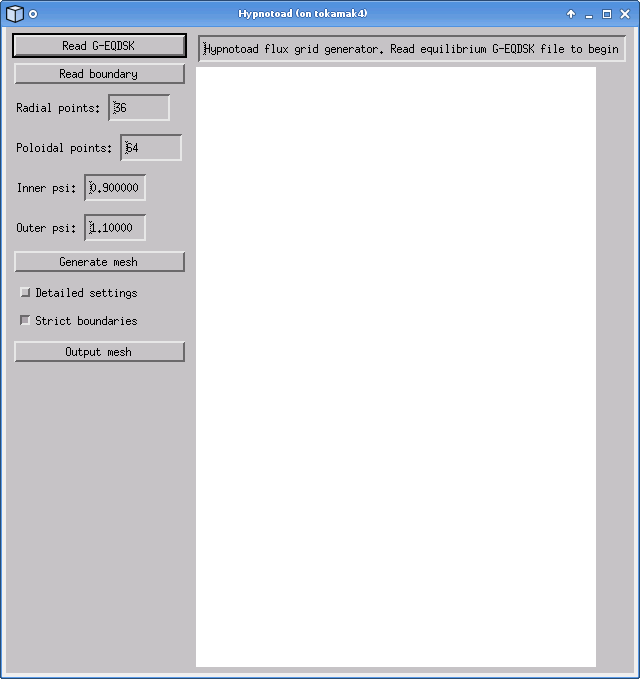
\includegraphics[width=0.5\paperwidth, keepaspectratio]{screen_0.png}
  \caption{Hypnotoad when started. On the left are a buttons to perform
    processing steps and change some settings,
    and on the right is the drawing area which will display the grid (white
    here, but might be black).
    At the top is a status area which will display text like error messages.}
  \label{fig:screen_0}
\end{figure}
\clearpage

First load the equilibrium file, which must be a G-EQDSK format file
(as output by EFIT). Click on the top button ``Read G-EQDSK'' which will
then ask for the file name as shown in Figure~\ref{fig:screen_1}.
\begin{figure}[h!]
  \centering
  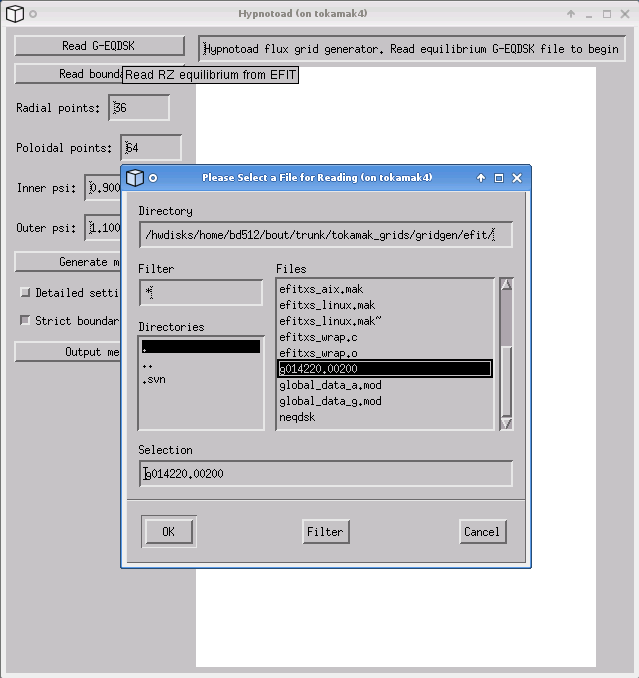
\includegraphics[width=0.5\paperwidth, keepaspectratio]{screen_1.png}
  \caption{Open a G-EQDSK formatted file. For this example we'll be using
    the MAST equilibrium file \file{g014220.00200} as shown, which is included
    in the BOUT++ repository (in the \file{gridgen/efit/} directory)}
  \label{fig:screen_1}
\end{figure}
\clearpage

If the file reading is successful then the grid will be displayed as shown
in Figure~\ref{fig:screen_2}.
\begin{figure}[h!]
  \centering
  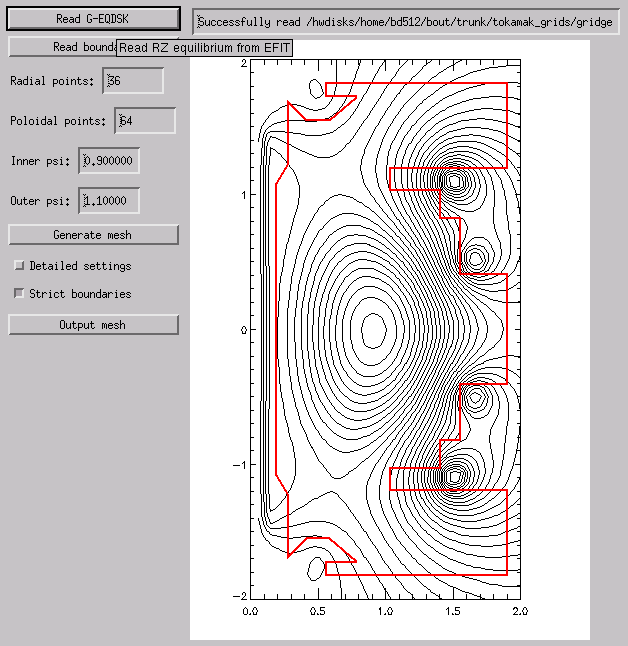
\includegraphics[width=0.5\paperwidth, keepaspectratio]{screen_2.png}
  \caption{If an equilibrium is read successfully then some psi contours
    are plotted in black, and if a boundary is defined then this is plotted
    as a thick red line. This equilibrium has a (slightly) lower double null
(LDN) configuration.}
  \label{fig:screen_2}
\end{figure}
Flux-surfaces of $\psi$ are shown in black, but these are just arbitrarily
chosen: there is no attempt to identify separatrices at this point. In red
is the boundary from the G-EQDSK file. Some G-EQDSK files don't specify
a boundary, and whilst it's possible to generate grids without one, the
result is usually not very good. If this is the case then no boundary will
appear, and the status box will contain a warning about missing boundary.
To read the boundary from a different
G-EQDSK file, click on the second button down labelled``Read boundary''.

Once you've got an equilibrium and boundary, enter the number of radial and
poloidal points you'd like in the final mesh into the boxes on the left, along
with the maximum range of normalised psi (0 = magnetic axis, 1 = innermost
separatrix). If this range is too large then it will be reduced automatically.

\clearpage
Clicking on ``Generate mesh'' runs the grid generator (in \file{create\_grid.pro})
the detailed of which are given in more detail in the following chapters.
Initially the x-points are located, and those which are inside the boundary and the range of psi specified are selected. These are then refined and analysed to
determine the directions corresponding to the divertor legs and the core
separatrices. Constant psi surfaces are followed to the target plates.
Figure~\ref{fig:screen_3} shows these lines and the initial attempt at
meshing the lower left divertor leg. Note that this meshing won't always
start at the lower left: Meshing starts from the innermost x-point
(i.e. the one with normalised $\psi = 1$) and proceeds clockwise around the
domain. For an Upper Double Null (UDN) configuration
the meshing therefore starts at the top right (outer upper divertor leg).
\begin{figure}[h!]
  \centering
\subfigure[Initial steps in generating the grid. X-points are found and the legs traced to the boundary. Regions are meshed and intersections with the boundary found (where blue lines are drawn to the origin)]{
  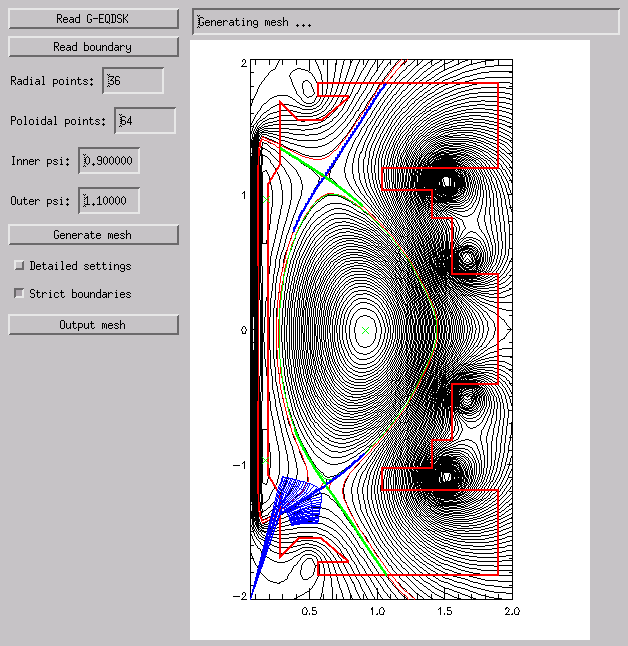
\includegraphics[width=0.35\paperwidth, keepaspectratio]{screen_3.png}
  \label{fig:screen_3}
}
\subfigure[Finished mesh with regions colored (black=1, red=2, green=3, blue=4, turquoise=5, purple=6)]{
  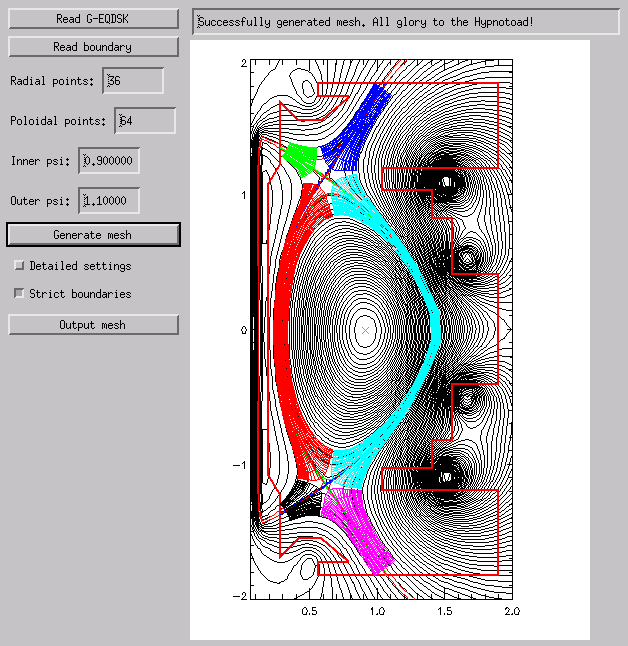
\includegraphics[width=0.35\paperwidth, keepaspectratio]{screen_4.png}
  \label{fig:screen_4}
}
\caption{Generating a mesh}
\label{fig:creategrid}
\end{figure}
You can adjust the settings and re-generate the mesh if needed. The switch
called ``Strict boundaries'' determines whether grid points are allowed to
cross the boundary. If this is switched off, the divertor legs will still end
at the boundary, but the radial mesh is allowed to cross the boundary.

\clearpage

Once you're happy with the mesh, click on ``Output mesh'' to create a
grid file for input to BOUT/BOUT++. This will prompt for a file to write,
and if you're overwriting a file it will ask you to confirm. 
\begin{figure}[h!]
  \centering
  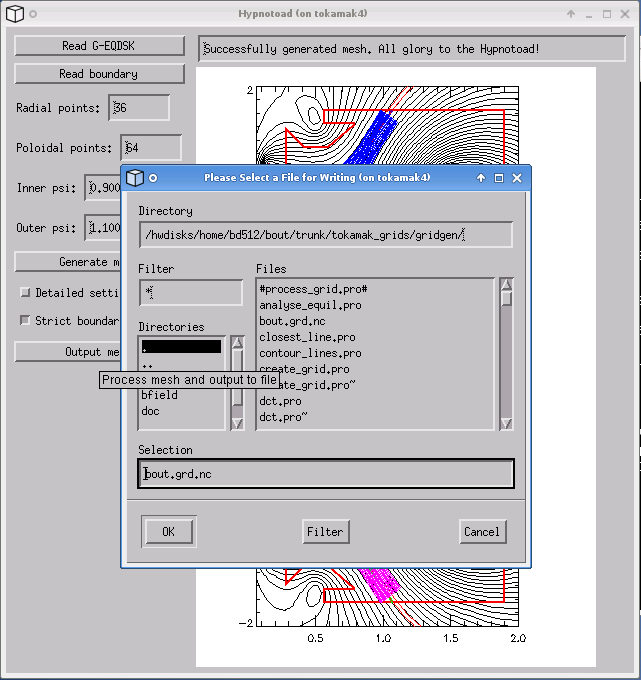
\includegraphics[width=0.5\paperwidth, keepaspectratio]{screen_5.png}
  \caption{Choosing name of output grid file}
  \label{fig:screen_5}
\end{figure}

Whereas mesh generation is automatic, turning a mesh into something which
can be used for simulations usually requires some user intervention. This
is mainly about checking that the equilibrium is reasonably good and that
the pressure and current profiles look sensible. If these are not good then
the simulation could have numerical problems, or just produce results which
are not correct.

\clearpage

Firstly the pressure gradient is calculated using 
\[
\mu_0\hthe\deriv{P}{x} = -\Bp\deriv{}{x}\left(\Bp\hthe\right) -\Bt\hthe\deriv{\Bt}{x} - \frac{\Bt^2\hthe}{R}\deriv{R}{x}
\]
(see \ref{sec:jxb_fac}) for derivation. $\hthe$ is calculated by measuring the
geometric distance between points, $\Bt$ from the $f\left(\psi\right)$ profile,
and $\Bp$ from derivatives of $\psi$ (done in \file{create\_mesh.pro} using DCTs). This calculated pressure is compared to the pressure profile from the
G-EQDSK file as shown in Figure~\ref{fig:screen_6}.
\begin{figure}[h!]
  \centering
  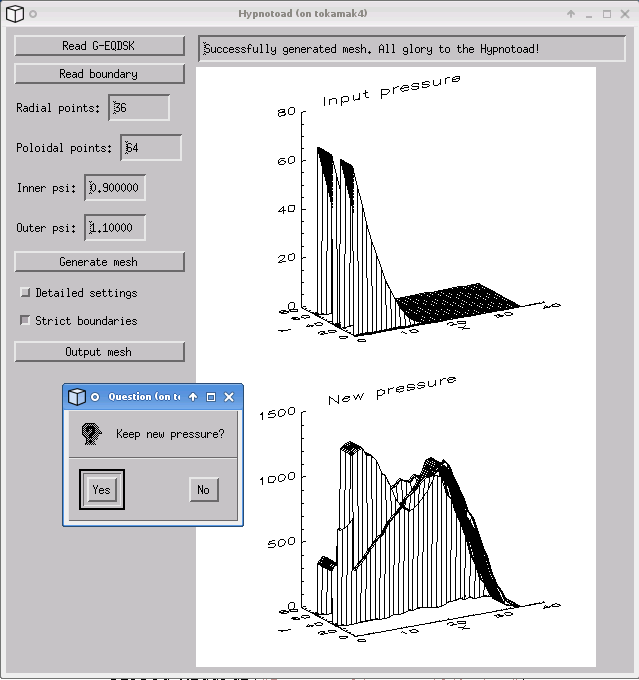
\includegraphics[width=0.5\paperwidth, keepaspectratio]{screen_6.png}
  \caption{Calculating pressure from force balance}
  \label{fig:screen_6}
\end{figure}

\clearpage
\begin{figure}[h!]
  \centering
\subfigure[]{
  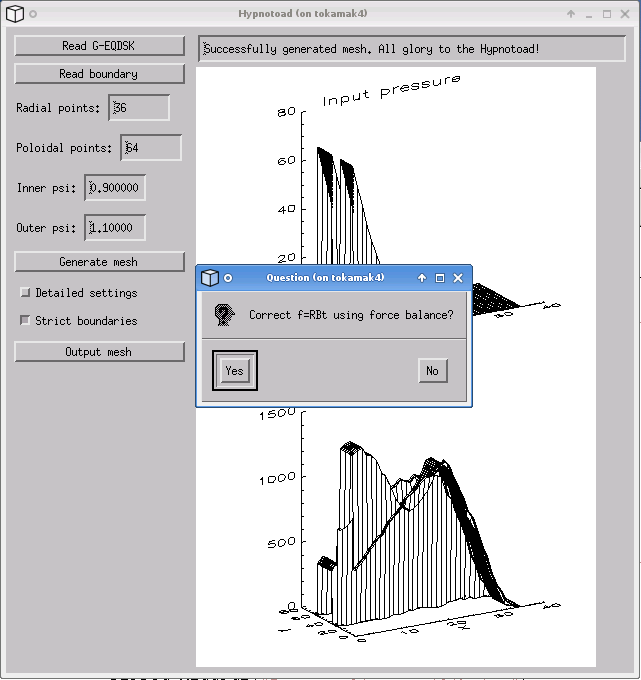
\includegraphics[width=0.35\paperwidth, keepaspectratio]{screen_7.png}
  \label{fig:screen_7}
}
\subfigure[result]{
  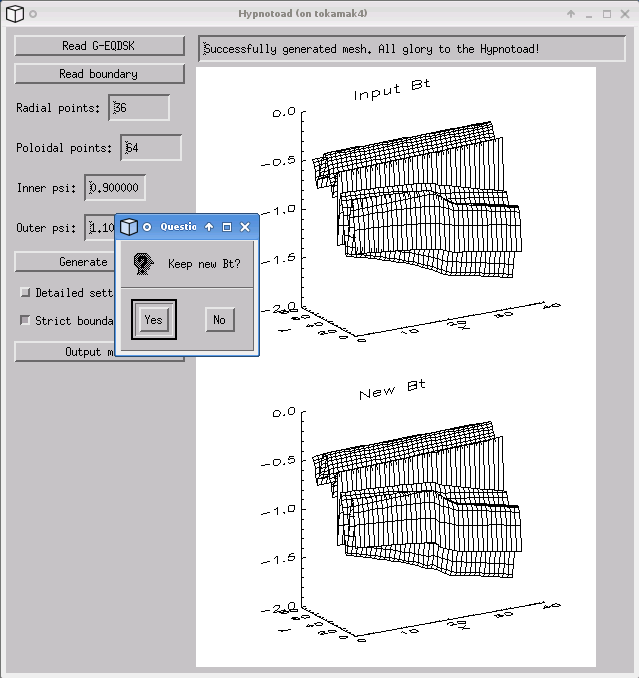
\includegraphics[width=0.35\paperwidth, keepaspectratio]{screen_8.png}
  \label{fig:screen_8}
}
\caption{Calculating $f=R\Bt$ from force balance}
\label{fig:rbt}
\end{figure}

\clearpage

\begin{figure}[h!]
  \centering
  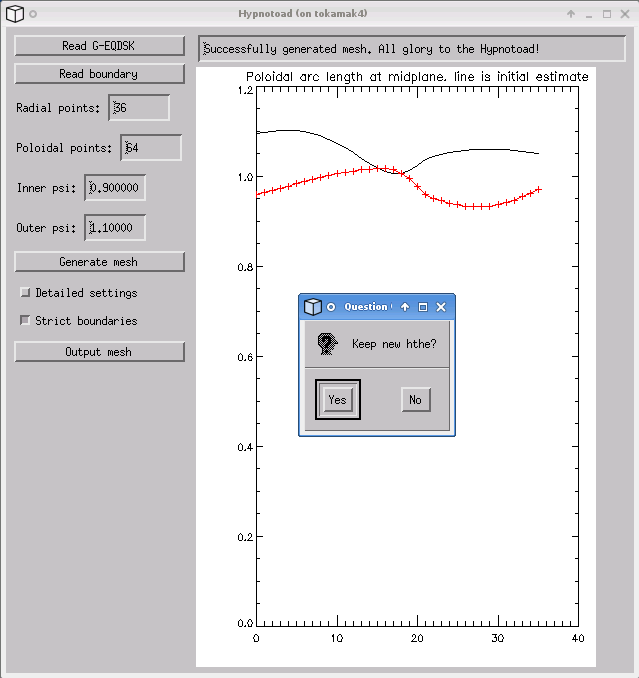
\includegraphics[width=0.5\paperwidth, keepaspectratio]{screen_9.png}
  \caption{Calculating poloidal arc length $\hthe$ from force balance}
  \label{fig:screen_9}
\end{figure}

\clearpage

\begin{figure}[h!]
  \centering
  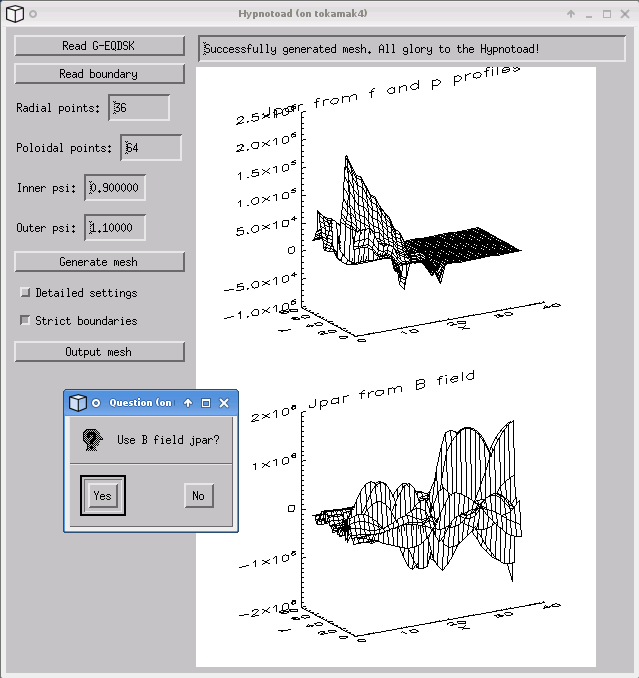
\includegraphics[width=0.5\paperwidth, keepaspectratio]{screen_10.png}
  \caption{Calculating $\Jpar$ from $f\left(\psi\right)$ and $p\left(\psi\right)$ (top), and from $\Vec{B}$ field (bottom)}
  \label{fig:screen_10}
\end{figure}

\clearpage

\begin{verbatim}
Generating plasma profiles:
  1. Flat temperature profile
  2. Flat density profile
  3. Te proportional to density
% Compiled module: GET_INTEGER.
Profile option:1
Setting flat temperature profile
% Compiled module: GET_FLOAT.
Temperature (eV):10
Maximum density (10^20 m^-3):     0.216518
Is this ok?y
Setting rmag =       1.46673
Setting bmag =       1.79263
Writing grid to file /hwdisks/home/bd512/bout/trunk/tokamak_grids/gridgen/bout.grd.nc
% Compiled module: FILE_OPEN.
% Compiled module: NCDF_EXISTS.
% Compiled module: FILE_WRITE.
% Compiled module: REVERSE_INDS.
% Compiled module: FILE_CLOSE.
DONE
\end{verbatim}

\section{Using the grid generator}

The function \code{create\_grid} takes a 2D array of $\psi$ values, and 
produces an orthogonal mesh aligned with the flux-surfaces.

Settings to control the resulting mesh are:
\begin{itemize}
\item \code{psi\_inner}, the normalised $\psi$ of the innermost flux surface. 
  This can be either a scalar or an array:
  \begin{itemize}
    \item \code{{\bf scalar}}: This value is used for the core and all PF regions
    \item \code{{\bf array[0]}}: The inner normalised $\psi$ for the core
    \item \code{{\bf array[1..n\_xpoint]}}: Inner $\psi$ to use for each PF region
      (see section~\ref{sec:numbering})
  \end{itemize}
\item \code{psi\_outer}, normalised $\psi$ of outermost surface. Can also be
  either a scalar or array:
  \begin{itemize}
  \item \code{{\bf scalar}}: This value is used for the core and all PF regions
  \item \code{{\bf array[0..(n\_xpoint-1)]}}: Outer normalised $\psi$ for each SOL region
    (one per x-point)
  \end{itemize}
\item \code{nrad} Number of radial grid points
  \begin{itemize}
  \item \code{{\bf scalar}}: Total number of radial grid points. Automatically divides this
    between regions.
  \item \code{{\bf array[0]}}: Number of radial grid points in the core
  \item \code{{\bf array[1..(n\_xpoint-1)]}}: Radial grid points between separatrices
    (going outwards from core to edge)
  \item \code{{\bf array[n\_xpoint]}}: Radial grid points outside last separatrix
  \end{itemize}
\item \code{npol} Number of poloidal grid points.
  \begin{itemize}
  \item \code{{\bf scalar}}: Total number of points. Divides between regions based on
    poloidal arc lengths
  \item \code{{\bf array[0..(3*n\_xpoint-1)]}}: Number of points in each poloidal region. 
    See section~\ref{sec:numbering} for numbering scheme.
  \end{itemize}
\item \code{rad\_peaking}
\item \code{pol\_peaking}
\end{itemize}

\section{DCT}

DCT of 2D NxM $f\left(x,y\right)$
\[
F\left(u, v\right) = \sqrt{\frac{2}{N}}\sqrt{\frac{2}{M}}\Lambda\left(u\right)\Lambda\left(v\right)\sum_{i=0}^{N-1}\sum_{j=0}^{M-1} f\left(i, j\right) \cos\left[\frac{\pi u}{2N}\left(2i+1\right)\right]\cos\left[\frac{\pi v}{2M}\left(2j+1\right)\right]
\]
where $\Lambda\left(i\right) = 1/\sqrt{2}$ for $i=0$, and $\Lambda\left(i\right) = 1$ otherwise
 
\section{Finding critical points}

To find x- and o-points, 

\section{Region numbering}
\label{sec:numbering}


\section{Separatrices}

Having found the x-point locations, the separatrices need to be found.
First step is to calculate the lines going through the x-point:

Close to an x-point, approximate the change in $\psi$ by
\[
\delta\psi = \frac{1}{2}\psi_{xx} x^2 + \frac{1}{2}\psi_{yy}y^2 + \psi_{xy} xy
\]

The two lines through the x-point are then given by where this is zero:

\[
\frac{1}{2}\psi_{yy}y^2 + \psi_{xy}xy + \frac{1}{2}\psi_{xx} x^2 = 0
\]
Which has the solution
\[
y = \frac{ -\psi_{xy}x \pm \sqrt{\psi_{xy}^2x^2 - \psi_{yy}\psi_{xx}x^2}}{\psi_{yy}}
\]
i.e.
\[
y = \frac{1}{\psi_{yy}}\left(-\psi_{xy} \pm \sqrt{\psi_{xy}^2 - \psi_{yy}\psi_{xx}}\right)x
\]
Note that if $\psi_{yy} = 0$ then the solutions are $x = 0$ and $y = -\frac{\psi_{xx}}{2\psi_{xy}}x$

\section{Differential geometry}

This section contains derivations of useful quantities or expressions
(like force balance) in flux and field-aligned coordinate systems.

\subsection{Toroidal coordinates}

Orthogonal toroidal coordinate system $\left(\psi, \theta, \zeta\right)$, 
where $\psi$ is the poloidal flux, $\theta$ the poloidal angle
(from $0$ to $2\pi$), and $\zeta$ the toroidal angle (also $0$ to $2\pi$).
The magnitudes of the unit vectors are
\begin{equation}
\left|\mathbf{e}_\psi\right| = \frac{1}{R\left|B_p\right|} \qquad
\left|\mathbf{e}_\theta\right| = h_\theta \qquad
\left|\mathbf{e}_\zeta\right| = R
\label{eq:fluxmags}
\end{equation}
The coordinate system is right handed, so $\mathbf{\hat{e}_\psi\times\hat{e}_\theta = \hat{e}_\zeta}$,
$\mathbf{\hat{e}_\psi\times\hat{e}_\zeta = -\hat{e}_\theta}$ and $\mathbf{\hat{e}_\theta\times\hat{e}_\zeta = \hat{e}_\psi}$. The metric coefficients are
\begin{equation}
g_{\psi\psi} = \frac{1}{\left(R\left|B_p\right|\right)^2} \qquad
g_{\theta\theta} = h_\theta^2 \qquad
g_{\zeta\zeta} = R^2
\end{equation}
and the magnitudes of the reciprocal vectors are therefore
\begin{equation}
\left|\nabla\psi\right| = R\left|B_p\right| \qquad
\left|\nabla\theta\right| = \frac{1}{h_\theta} \qquad
\left|\nabla\zeta\right| = \frac{1}{R}
\label{eq:fluxmags2}
\end{equation}

Because the coordinate system is orthogonal, $g^{ii} = 1/g_{ii}$ and so the cross-products can be calculated as
\begin{eqnarray*}
\nabla\psi\times\nabla\theta = &\mathbf{e^\psi\times e^\theta} = 
g^{\psi\psi}\mathbf{e}_\psi\times g^{\theta\theta}\mathbf{e}_\theta \nonumber \\
= & g^{\psi\psi}g^{\theta\theta}h_\psi h_\theta\mathbf{\hat{e}_\psi\times\hat{e}_\theta} \nonumber \\
= &\frac{1}{h_\psi h_\theta}\mathbf{\hat{e}}_\zeta 
= \frac{R\left|B_p\right|}{h_\theta}\mathbf{\hat{e}}_\zeta
\end{eqnarray*}
Similarly, 
\[
\nabla\psi\times\nabla\zeta = -\left|B_p\right|\mathbf{\hat{e}}_\theta \qquad
\nabla\theta\times\nabla\zeta = \frac{1}{Rh_\theta}\mathbf{\hat{e}}_\psi = \frac{1}{h_\theta R^2\left|\Bp\right|}\nabla \psi
\]

Field-aligned coordinates $(x,y,z)$ are defined by:

\begin{eqnarray}
x &=& \sbp\left(\psi - \psi_0\right) \\ 
y &=& \theta \\
z &=& \sbp\left[\zeta - \int_{\theta_0}^{\theta}\nu\left(\psi, \theta\right)d\theta\right]
\label{eq:coordtransform}
\end{eqnarray}
Where $\nu$ is the local field-line pitch given by
\begin{equation}
\nu\left(\psi, \theta\right) = \frac{\mathbf{B}\cdot\nabla\zeta}{\mathbf{B}\cdot\nabla\theta} = \frac{\Bt\hthe}{\Bp R}
\end{equation}

and the \sbp is the sign of the poloidal field $\Bp / \left|\Bp\right|$. This means $x$ always increases from core to edge

The contravariant basis vectors are therefore
\begin{eqnarray*}
\nabla x &=& \sbp \nabla \psi \\
\nabla y &=& \nabla \theta \\
\nabla z &=& \sbp \left( \nabla\zeta - \left[\int_{\theta_0}^\theta\deriv{\nu\left(\psi, \theta\right)}{\psi} d\theta\right] \nabla\psi - \nu\left(\psi, \theta\right)\nabla\theta \right)
\end{eqnarray*}

The term in square brackets is the integrated local shear:
\[
I = \int_{y_0}^y\frac{\partial\nu\left(x, y\right)}{\partial\psi}dy
\]

\subsection{Metrics}

Magnetic field is defined as:
\[
\mathbf{B} = \nabla z\times \nabla x
\]
The contravariant components of this are then
\begin{equation}
B^y = \frac{\Bp}{\hthe} \qquad B^x = B^z = 0
\label{eq:B_contravariant}
\end{equation}
i.e. $\Bvec$ can be written as
\begin{equation}
\Bvec = \frac{\Bp}{\hthe}\mathbf{e}_y
\label{eq:Bvec_cont}
\end{equation}
and the covariant components calculated using $g_{ij}$ as
\begin{equation}
B_x = \Bt I R \qquad B_y = \frac{B^2 \hthe}{\Bp} \qquad B_z = \Bt R
\label{eq:B_covariant}
\end{equation}

The Jacobian of this coordinate system is
\[
J^{-1} \equiv \left(\nabla x\times\nabla y\right)\cdot\nabla z = \Bp / \hthe
\]

The contravariant metric tensor is given by:
\[
g^{ij} \equiv \Vec{e}^i \cdot\Vec{e}^j \equiv \nabla u^i \cdot \nabla u^j = \left(\begin{array}{ccc}
\left(R\Bp\right)^2 & 0 & -I\left(R\Bp\right)^2 \\
0 & 1 / \hthe^2 & -\sbp\nu / \hthe^2 \\
-I\left(R\Bp\right)^2 & -\sbp\nu / \hthe^2 & I^2\left(R\Bp\right)^2 + B^2 / \left(R\Bp\right)^2 \end{array} \right)
\]
and the covariant metric tensor:
\[
g_{ij} \equiv \Vec{e}_i \cdot\Vec{e}_j = \left(\begin{array}{ccc}
I^2 R^2 + 1 / \rbpsq & \sbp\Bt\hthe I R / \Bp & I R^2 \\
\sbp\Bt\hthe I R / \Bp & B^2\hthe^2 / \Bp^2 & \sbp\Bt\hthe R / \Bp \\
I R^2 & \sbp\Bt\hthe R / \Bp & R^2 \end{array} \right)
\]

\subsection{Differential operators}

The derivative along the unperturbed magnetic field is given by
\[
\nabla_{||0}A \equiv \Vec{b}_0 \cdot\nabla A = \frac{\Bp}{B\hthe}\deriv{A}{y}
\]
Using equation (\ref{eq:general_laplacian}), the laplacian operator is given by
\begin{eqnarray}
\nabla^2 = &\frac{\partial^2}{\partial x^2}\left|\nabla x\right|^2 + 
\frac{\partial^2}{\partial y^2}\left|\nabla y\right|^2 + 
\frac{\partial^2}{\partial z^2}\left|\nabla z\right|^2 \nonumber \\
&-2\frac{\partial^2}{\partial x\partial z}I\left(RB_p\right)^2 - 2\frac{\partial^2}{\partial y\partial z}\frac{\nu}{h_\theta^2}\\
&+\frac{\partial}{\partial x}\nabla^2x + \frac{\partial}{\partial y}\nabla^2y + \frac{\partial}{\partial z}\nabla^2z \nonumber
\end{eqnarray}
Using equation (\ref{eq:laplace_expand}) for $\nabla^2x = -\Gamma^x$ etc, the values are
\begin{equation}
\nabla^2x = \frac{B_p}{h_\theta}\frac{\partial}{\partial x}\left(h_\theta R^2B_p\right) \qquad
\nabla^2y = \frac{B_p}{h_\theta}\frac{\partial}{\partial y}\left(\frac{1}{B_ph_\theta}\right)
\end{equation}
\[
\nabla^2z = -\frac{B_p}{h_\theta}\left[\frac{\partial}{\partial x}\left(IR^2B_ph_\theta\right) + \frac{\partial}{\partial y}\left(\frac{\nu}{B_ph_\theta}\right)\right]
\]

\subsection{$J\times B$ in field-aligned coordinates}
\label{sec:jxb_fac}

Components of the magnetic field in field-aligned coordinates:
\[
B^y = \frac{\Bp}{\hthe} \qquad B^x = B^z = 0
\]
and
\[
B_x = \sbp\Bt I R \qquad B_y = \frac{B^2\hthe}{\Bp} \qquad B_z = \sbp\Bt R
\]

Calculate current $\Jvec = \frac{1}{\mu}\Curl{\Bvec}$

\[
\left(\Curl{\Bvec}\right)^x = \frac{1}{J}\left(\deriv{B_z}{y} - \deriv{B_y}{z}\right) = 0
\]
since $\Bt R$ is a flux-surface quantity, and $\Bvec$ is axisymmetric.
\begin{eqnarray*}
\left(\Curl{\Bvec}\right)^y &=& -\sbp\frac{\Bp}{\hthe}\deriv{}{x}\left(\Bt R\right) \\
\left(\Curl{\Bvec}\right)^z &=& \frac{\Bp}{\hthe}\left[\deriv{}{x}\left(\frac{B^2\hthe}{\Bp}\right) - \sbp\deriv{}{y}\left(\Bt I R\right)\right]
\end{eqnarray*}
The second term can be simplified, again using $\Bt R$ constant on flux-surfaces:
\[
\deriv{}{y}\left(\Bt I R\right) = \Bt R\deriv{\nu}{x} \qquad \nu = \frac{\hthe\Bt}{R\Bp}
\]
From these, calculate covariant components:
\begin{eqnarray}
\left(\Curl{\Bvec}\right)_x &=& -\Bt I R \deriv{}{x}\left(\Bt R\right) + \frac{IR^2\Bp}{\hthe}\left[\deriv{}{x}\left(\frac{B^2\hthe}{\Bp}\right) - \sbp\Bt R\deriv{\nu}{x}\right] \nonumber\\
\left(\Curl{\Bvec}\right)_y &=& -\sbp\frac{B^2\hthe}{\Bp}\deriv{}{x}\left(\Bt R\right) + \sbp\Bt R\left[\deriv{}{x}\left(\frac{B^2\hthe}{\Bp}\right) - \sbp\Bt R\deriv{\nu}{x}\right] \label{eq:curlb_y}\\
\left(\Curl{\Bvec}\right)_z &=& -\Bt R\deriv{}{x}\left(\Bt R\right) + \frac{R^2\Bp}{\hthe}\left[\deriv{}{x}\left(\frac{B^2\hthe}{\Bp}\right) - \sbp\Bt R\deriv{\nu}{x}\right] \nonumber
\end{eqnarray}
Calculate $\Jvec\times\Bvec$ using
\begin{equation}
\mathbf{e}^i = \frac{1}{J}\left(\mathbf{e}_j \times \mathbf{e}_k\right) \qquad \mathbf{e}_i = J\left(\mathbf{e}^j \times \mathbf{e}^k\right) \qquad i,j,k \texttt{ cyc } 1,2,3
\label{eq:cross_relation}
\end{equation}
gives 
\begin{eqnarray*}
\mu_0 \left(\Jvec\times\Bvec\right)^x &=& \frac{1}{J}\left[\left(\Curl{\Bvec}\right)_y B_z - \left(\Curl{\Bvec}\right)_z B_y \right]\\
&=& -\frac{\Bp^3 R^2}{\hthe}\left[\deriv{}{x}\left(\frac{B^2\hthe}{\Bp}\right) - \sbp\Bt R\deriv{\nu}{x}\right]
\end{eqnarray*}

Covariant components of $\nabla P$:
\[
\left(\nabla P\right)_x = \deriv{P}{x} \qquad \left(\nabla P\right)_y = \left(\nabla P\right)_z = 0
\]
and contravariant:
\[
\left(\nabla P\right)^x = \rbpsq\deriv{P}{x} \qquad \left(\nabla P\right)^y = 0 \qquad \left(\nabla P\right)^z = -I\rbpsq\deriv{P}{x}
\]
Hence equating contravariant x components of $\Jvec\times\Bvec = \nabla P$,
\begin{equation}
\deriv{}{x}\left(\frac{B^2\hthe}{\Bp}\right) - \sbp\Bt R\deriv{}{x}\left(\frac{\Bt\hthe}{R\Bp}\right) + \frac{\mu_0\hthe}{\Bp}\deriv{P}{x} = 0
\label{eq:xbalance}
\end{equation}
Use this to calculate $\hthe$ profiles (need to fix $\hthe$ at one radial location).

Close to x-points, the above expression becomes singular, so a better way to write it is:
\[
\deriv{}{x}\left(B^2\hthe\right) - \hthe\Bp\deriv{\Bp}{x} - \sbp \Bt R\deriv{}{x}\left(\frac{\Bt\hthe}{R}\right) + \mu_0\hthe\deriv{P}{x} = 0
\]

For solving force-balance by adjusting $P$ and $f$ profiles, the form used is
\[
\Bt\hthe\deriv{\Bt}{x} + \frac{\Bt^2\hthe}{R}\deriv{R}{x} + \mu_0\hthe\deriv{P}{x} = -\Bp\deriv{}{x}\left(\Bp\hthe\right)
\]
A quick way to calculate f is to rearrange this to:
\[
\deriv{\Bt}{x} = \Bt\left[-\frac{1}{R}\deriv{R}{x}\right] + \frac{1}{\Bt}\left[-\mu_0\deriv{P}{x} - \deriv{\Bp}{\hthe}\deriv{}{x}\left(\Bp\hthe\right)\right]
\]
and then integrate this using LSODE. This is done in the \code{solve\_f} function in \file{process\_grid.pro}

\subsection{Parallel current}

\[
J_{||} = \mathbf{b}\cdot\Jvec \qquad b^y = \frac{\Bp}{B\hthe}
\]
and from equation \ref{eq:curlb_y}:
\[
J_y = \frac{1}{\mu_0}\left\{-\frac{B^2\hthe}{\Bp}\deriv{}{x}\left(\Bt R\right) + \Bt R\left[\deriv{}{x}\left(\frac{B^2\hthe}{\Bp}\right) - \Bt R\deriv{\nu}{x}\right]\right\}
\]
since $J_{||} = b^yJ_y$,
\[
\mu_0 J_{||} =\frac{\Bp\Bt R}{B\hthe}\left[\deriv{}{x}\left(\frac{B^2\hthe}{\Bp}\right) - \Bt R\deriv{\nu}{x}\right] - B\deriv{}{x}\left(\Bt R\right)
\]

\subsection{Curvature}

For reduced MHD, need to calculate curvature term $\mathbf{b}\times\mathbf{\kappa}$, where
$\mathbf{\kappa} = \left(\bvec\cdot\nabla\right)\bvec = -\mathbf{b}\times\left(\nabla\times\mathbf{b}\right)$. Re-arranging, this becomes:
\[
\mathbf{b}\times\mathbf{\kappa} = \nabla\times\mathbf{b} - \mathbf{b}\left(\mathbf{b}\cdot\left(\nabla\times\mathbf{b}\right)\right)
\]
Components of $\nabla\times\mathbf{b}$ are:
\begin{eqnarray*}
\left(\nabla\times\mathbf{b}\right)^x &=& \frac{\Bp}{\hthe}\deriv{}{y}\left(\frac{\Bt R}{B}\right) \\
\left(\nabla\times\mathbf{b}\right)^y &=& -\frac{\Bp}{\hthe}\deriv{}{x}\left(\frac{\Bt R}{B}\right) \\
\left(\nabla\times\mathbf{b}\right)^z &=& \frac{\Bp}{\hthe}\deriv{}{x}\left(\frac{B\hthe}{\Bp}\right) - \frac{\Bp\Bt R}{\hthe B}\deriv{\nu}{x} - I\frac{\Bp}{\hthe}\deriv{}{y}\left(\frac{\Bt R}{B}\right) \\
\end{eqnarray*}

giving:
\begin{eqnarray}
\mathbf{\kappa} &=& -\frac{B_\theta}{B h_\theta}\left[\deriv{}{x}\left(\frac{B h_\theta}{B_\theta}\right) - \sbp\deriv{}{y}\left(\frac{B_\zeta I R}{B}\right)\right]\nabla x \nonumber \\
&+& \sbp\frac{B_\theta}{B h_\theta}\deriv{}{y}\left(\frac{B_\zeta R}{B}\right)\nabla z
\label{eq:curvature}
\end{eqnarray}

\[
\mathbf{b}\cdot\left(\nabla\times\mathbf{b}\right) = -B\deriv{}{x}\left(\frac{\Bt R}{B}\right) + \frac{\Bt\Bp R}{B\hthe}\deriv{}{x}\left(\frac{B\hthe}{\Bp}\right) - \frac{\Bp\Bt^2R^2}{\hthe B^2}\deriv{\nu}{x}
\]

therefore,
\begin{eqnarray*}
\left(\mathbf{b}\times\mathbf{\kappa}\right)^x &=& \frac{\Bp}{\hthe}\deriv{}{y}\left(\frac{\Bt R}{B}\right) = -\frac{\Bp\Bt R}{\hthe B^2}\deriv{B}{y} \\
\left(\mathbf{b}\times\mathbf{\kappa}\right)^y &=& \frac{\Bp^2\Bt^2 R^2}{B^3\hthe^2}\deriv{\nu}{x} - \frac{\Bp^2\Bt R}{B^2\hthe^2}\deriv{}{x}\left(\frac{B\hthe}{\Bp}\right) \\
\left(\mathbf{b}\times\mathbf{\kappa}\right)^z &=& \frac{\Bp}{\hthe}\deriv{}{x}\left(\frac{B\hthe}{\Bp}\right) - \frac{\Bp\Bt R}{\hthe B}\deriv{\nu}{x} - I\left(\mathbf{b}\times\mathbf{\kappa}\right)^x
\end{eqnarray*}
Using equation~\ref{eq:xbalance}:
\[
B\deriv{}{x}\left(\frac{B\hthe}{\Bp}\right) + \frac{B\hthe}{\Bp}\deriv{B}{x} - \Bt R\deriv{}{x}\left(\frac{\Bt\hthe}{R\Bp}\right) + \frac{\mu_0\hthe}{\Bp}\deriv{P}{x} = 0
\]
we can re-write the above components as:
\begin{eqnarray*}
\left(\mathbf{b}\times\mathbf{\kappa}\right)^y &=& \frac{\Bp\Bt R}{B^2\hthe}\left[\frac{\mu_0}{B}\deriv{P}{x} + \deriv{B}{x}\right] \\
\left(\mathbf{b}\times\mathbf{\kappa}\right)^z &=& -\frac{\mu_0}{B}\deriv{P}{x} - \deriv{B}{x} - I\left(\mathbf{b}\times\mathbf{\kappa}\right)^x
\end{eqnarray*}

\subsection{Curvature of single line}

The curvature vector can be calculated from the field-line toroidal
coordinates $\left(R,Z,\phi\right)$ as follows. The line element
is given by
\[
d\Vec{r} = dR\Rvec + dZ\Zvec + Rd\phi\phivec
\]
Hence the tangent vector is
\[
\hat{\Vec{T}} \equiv \dd{\Vec{r}}{s} = \dd{R}{s}\Rvec + \dd{Z}{s}\Zvec + R\dd{\phi}{s}\phivec
\]
where $s$ is the distance along the field-line. From this, the curvature vector
is given by
\begin{eqnarray*}
\kvec \equiv \dd{\Vec{T}}{s} &=& \ddd{R}{s}\Rvec + \dd{R}{s}\dd{\phi}{s}\phivec \\
&+& \ddd{Z}{s}\Zvec \\
&+& \dd{R}{s}\dd{\phi}{s}\phivec + R\ddd{\phi}{s}\phivec - R\left(\dd{\phi}{s}\right)^2 \Rvec
\end{eqnarray*}
i.e.
\begin{equation}
\kvec = \left[\ddd{R}{s} - R\left(\dd{\phi}{s}\right)^2\right]\Rvec + \ddd{Z}{s}\Zvec + \left[2\dd{R}{s} + R\ddd{\phi}{s}\right]\phivec
\label{eq:kappaline}
\end{equation}
Want the components of $\Vec{b}\times\kvec$, and since the vector $\Vec{b}$
is just the tangent vector $\Vec{T}$ above, this can be written using the
cross-products
\[
\Rvec\times\Zvec = -\phivec \qquad \phivec\times\Zvec = \Rvec \qquad \Rvec\times\phivec = \Zvec
\]
This vector must then be dotted with $\nabla\psi$, $\nabla\theta$, and $\nabla\phi$. This is done by writing these vectors in cylindrical coordinates:
\begin{eqnarray*}
\nabla\psi &=& \deriv{\psi}{R}\hat{\Vec{R}} + \deriv{\psi}{Z}\hat{\Vec{Z}} \\
\nabla\theta &=& \frac{1}{\Bp\hthe}\nabla\phi\times\nabla\psi = \frac{1}{R\Bp\hthe}\left(\deriv{\psi}{Z}\hat{\Vec{R}} - \deriv{\psi}{R}\hat{\Vec{Z}}\right) \\
\end{eqnarray*}

An alternative is to use
\[
\bvec \times \nabla\phi = \frac{\sbp}{BR^2}\nabla\psi
\]
and that the tangent vector $\Vec{T} = \bvec$. This gives
\begin{equation}
\nabla\psi = \sbp BR\left[\frac{dR}{ds}\Vec{Z} - \frac{dZ}{ds}\Vec{R}\right] 
\label{eq:flinegradpsi}
\end{equation}
and so because $d\phi / ds = \Bt / \left(RB\right)$
\begin{equation}
\kvec\cdot\nabla\psi = \sbp BR\left[ \left( \frac{\Bt^2}{RB^2} - \ddd{R}{s}\right)\dd{Z}{s} + \ddd{Z}{s}\frac{dR}{ds} \right]
\label{eq:flinekappsi}
\end{equation}

Taking the cross-product of the tangent vector with the curvature in equation~\ref{eq:kappaline} above gives
\begin{eqnarray*}
  \bvec \times\kvec &=& \left[\frac{\Bt}{B}\ddd{Z}{s} - \dd{Z}{s}\left(2\dd{R}{s} + R\ddd{\phi}{s}\right)\right]\Vec{R} \\
  &+& \left[\dd{R}{s}\left(2\dd{R}{s} + R\ddd{\phi}{s}\right) - \frac{\Bt}{B}\left(\ddd{R}{s} - R\left(\dd{\phi}{s}\right)^2\right)\right]\Vec{Z} \\
  &+& \left[\dd{Z}{s}\left(\ddd{R}{s} - R\left(\dd{\phi}{s}\right)^2\right) - \dd{R}{s}\ddd{Z}{s}\right]\phivec
\end{eqnarray*}

The components in field-aligned coordinates can then be calculated:
\begin{eqnarray*}
\left(\bvec\times\kvec\right)^x &=& \sbp\left(\bvec\times\kvec\right)\cdot\nabla\psi \\
&=& \frac{R\Bp^2}{B}\left(2\dd{R}{s} + R\ddd{\phi}{s}\right) - R\Bt\left(\dd{R}{s}\ddd{R}{s} + \dd{Z}{s}\ddd{Z}{s}\right) + \frac{\Bt^3}{B^2}\dd{R}{s}
\end{eqnarray*}

\subsection{Curvature in toroidal coordinates}

In toroidal coordinates $\left(\psi,\theta,\phi\right)$, the $\bvec$ vector
is
\begin{eqnarray*}
\bvec &=& \frac{\Bp}{B}\ehat_\theta + \frac{\Bt}{B}\ehat_\phi \\
&=& \frac{\Bp\hthe}{B}\nabla\theta + \frac{R\Bt}{B}\nabla\phi
\end{eqnarray*}
The curl of this vector is
\begin{eqnarray*}
\left(\nabla\times\bvec\right)^\psi &=& \frac{1}{\sqrt{g}}\left(\deriv{b_\phi}{\theta} - \deriv{b_\theta}{\phi}\right) \\
\left(\nabla\times\bvec\right)^\theta &=& \frac{1}{\sqrt{g}}\left(\deriv{b_\psi}{\phi} - \deriv{b_\phi}{\psi}\right) \\
\left(\nabla\times\bvec\right)^\phi &=& \frac{1}{\sqrt{g}}\left(\deriv{b_\theta}{\psi} - \deriv{b_\psi}{\theta}\right)
\end{eqnarray*}
where $1/\sqrt{g} = \Bp/\hthe$. Therefore, in terms of unit vectors:
\[
\nabla\times\bvec = \frac{1}{R\hthe}\deriv{}{\theta}\left(\frac{R\Bt}{B}\right)\ehat_\psi - \Bp\deriv{}{\psi}\left(\frac{R\Bt}{B}\right)\ehat_\theta + \frac{\Bp R}{\hthe}\deriv{}{\psi}\left(\frac{\hthe\Bp}{B}\right)\ehat_\phi
\]

\subsection{$\psi$ derivative of $B$ field}

Needed to calculate magnetic shear, and one way to get the curvature.
The simplest way is to use finite differencing, but there is another way
using local derivatives (implemented using DCT).
\[
\Bp = \frac{\left|\nabla\psi\right|}{R} = \frac{1}{R}\sqrt{\left(\deriv{\psi}{R}\right)^2 + \left(\deriv{\psi}{R}\right)^2}
\]
Using
\[
\nabla\Bp = \deriv{\Bp}{\psi}\nabla\psi + \deriv{\Bp}{\theta}\nabla\theta + \deriv{\Bp}{\phi}\nabla\phi
\]
we get
\[
\nabla\Bp \cdot\nabla\psi = \deriv{\Bp}{\psi}\left|\nabla\psi\right|^2
\]
and so
\[
\deriv{\Bp}{\psi} = \nabla\Bp \cdot\nabla\psi / \left(R\Bp\right)^2
\]
The derivatives of $\Bp$ in $R$ and $Z$ are:
\begin{eqnarray*}
\deriv{\Bp}{R} &=& -\frac{\Bp}{R} + \frac{1}{\Bp R^2}\left[\deriv{\psi}{R}\dderiv{\psi}{R} + \deriv{\psi}{Z}\frac{\partial^2\psi}{\partial R\partial Z}\right] \\
\deriv{\Bp}{Z} &=& \frac{1}{\Bp R^2}\left[\deriv{\psi}{Z}\dderiv{\psi}{Z} + \deriv{\psi}{R}\frac{\partial^2\psi}{\partial R\partial Z}\right]
\end{eqnarray*}

For the toroidal field, $\Bt = f/R$
\[
\deriv{\Bt}{\psi} = \frac{1}{R}\deriv{f}{\psi} - \frac{f}{R^2}\deriv{R}{\psi}
\]
As above, $\deriv{R}{\psi} = \nabla R \cdot\nabla\psi / \left(R\Bp\right)^2$,
and since $\nabla R\cdot\nabla R = 1$,
\[
\deriv{R}{\psi} = \deriv{\psi}{R} / \left(R\Bp\right)^2
\]
similarly,
\[
\deriv{Z}{\psi} = \deriv{\psi}{Z} / \left(R\Bp\right)^2
\]
and so the variation of toroidal field with $\psi$ is
\[
\deriv{\Bt}{\psi} = \frac{1}{R}\deriv{f}{\psi} - \frac{\Bt}{R^3\Bp^2}\deriv{\psi}{R}
\]

From the definition $B=\sqrt{\Bt^2 + \Bp^2}$, 
\[
\deriv{B}{\psi} = \frac{1}{B}\left(\Bt\deriv{\Bt}{\psi} + \Bp\deriv{\Bp}{\psi}\right)
\]

\subsection{Magnetic shear from $J\times B$}

Re-arranging the radial force balance equation~\ref{eq:xbalance} gives
\[
\frac{\Bp^2R}{\Bt}\deriv{\nu}{\psi} + \nu\left(\frac{2RB}{\Bt}\deriv{B}{\psi} + \frac{B^2}{\Bt}\deriv{R}{\psi} - \frac{B^2R}{\Bt^2}\deriv{\Bt}{\psi}\right) + \frac{\mu_0\hthe}{\Bp}\deriv{P}{\psi} = 0
\]

\subsection{Magnetic shear}

The field-line pitch is given by
\[
\nu = \frac{\hthe\Bt}{\Bp R}
\]
and so
\[
\deriv{\nu}{\psi} = \frac{\nu}{\hthe}\deriv{\hthe}{\psi} + \frac{\nu}{\Bt}\deriv{\Bt}{\psi} - \frac{\nu}{\Bp}\deriv{\Bp}{\psi} - \frac{\nu}{R}\deriv{R}{\psi}
\]
The last three terms are given in the previous section, but $\partial\hthe/\partial\psi$ needs to be evaluated

\subsection{$\psi$ derivative of $\hthe$}

From the expression for curvature \ref{eq:curvature}, and using $\nabla x \cdot \nabla \psi = \sbp \left(R\Bp\right)^2$ and $\nabla z\cdot\nabla \psi = -\sbp I \left(R\Bp\right)^2$

\begin{eqnarray*}
\kvec\cdot\nabla\psi &=& -\sbp \frac{\Bp}{B\hthe}\rbpsq\left[\deriv{}{x}\left(\frac{B\hthe}{\Bp}\right) - \sbp\deriv{}{y}\left(\frac{\Bt IR}{B}\right)\right] \\
&&- I\rbpsq \frac{\Bp}{B\hthe}\deriv{}{y}\left(\frac{\Bt R}{B}\right)
\end{eqnarray*}

The second and third terms partly cancel, and using $\deriv{I}{y} = \sbp \deriv{\nu}{x}$
\begin{eqnarray*}
  \frac{\kvec\cdot\nabla\psi}{\rbpsq} &=& -\sbp\frac{\Bp}{B\hthe}\deriv{}{x}\left(\frac{B\hthe}{\Bp}\right) + \sbp\frac{\Bp}{B\hthe}\frac{\Bt R}{B}\deriv{\nu}{x} \\
  &=& -\sbp\frac{\Bp}{B\hthe}\left[\deriv{}{x}\left(\frac{B\hthe}{\Bp}\right) - \frac{\Bt R}{B}\deriv{}{x}\left(\frac{\Bt\hthe}{\Bp R}\right)\right] \\
  &=& -\sbp\frac{\Bp}{B\hthe}\left[\hthe\deriv{}{x}\left(\frac{B}{\Bp}\right) - \hthe\frac{\Bt R}{B}\deriv{}{x}\left(\frac{\Bt}{\Bp R}\right) + \frac{B^2}{B\Bp}\deriv{\hthe}{x} - \frac{\Bt^2}{B\Bp}\deriv{\hthe}{x}\right] \\
  &=& -\sbp \frac{\Bp}{B^2\hthe}\deriv{\hthe}{x} - \sbp\frac{\Bp}{B^2}\left[B\deriv{}{x}\left(\frac{B}{\Bp}\right) - \Bt R\deriv{}{x}\left(\frac{\Bt}{\Bp R}\right)\right]
\end{eqnarray*}
Writing
\begin{eqnarray*}
B\deriv{}{x}\left(\frac{B}{\Bp}\right) &=& \deriv{}{x}\left(\frac{B^2}{\Bp}\right) - \frac{B}{\Bp}\deriv{B}{x} \\
\Bt R\deriv{}{x}\left(\frac{\Bt}{\Bp R}\right) &=& \deriv{}{x}\left(\frac{\Bt^2}{\Bp}\right) - \frac{\Bt}{\Bp R}\deriv{}{x}\left(\Bt R\right)
\end{eqnarray*}
and using $B\deriv{B}{x} = \Bt\deriv{\Bt}{x} + \Bp\deriv{\Bp}{x}$, this simplifies to give
\begin{equation}
\frac{\kvec\cdot\nabla\psi}{\rbpsq} = -\sbp\frac{\Bp^2}{B^2\hthe}\deriv{\hthe}{x} - \sbp\frac{\Bt^2}{B^2 R}\deriv{R}{x}
\label{eq:dhdpsi}
\end{equation}

This can be transformed into an expression for $\deriv{\hthe}{x}$ involving only derivatives along
field-lines. 
Writing $\nabla R = \deriv{R}{\psi}\nabla\psi + \deriv{R}{\theta}\nabla\theta$, 
\[
\nabla R \cdot \nabla\psi = \deriv{R}{\psi}\rbpsq
\]
Using \ref{eq:flinegradpsi}, 
\[
\nabla\psi \cdot \nabla R = -\sbp B R\frac{dZ}{ds}
\]
and so
\[
\deriv{R}{x} = -\frac{BR}{\rbpsq}\frac{dZ}{ds}
\]
Substituting this and equation \ref{eq:flinekappsi} for $\kvec\cdot\nabla\psi$ into equation~\ref{eq:dhdpsi}
the $\deriv{R}{x}$ term cancels with part of the $\kvec\cdot\nabla\psi$ term, simplifying to
\begin{equation}
\deriv{\hthe}{x} = -\hthe\frac{B^3R}{\Bp^2\rbpsq}\left[\frac{d^2Z}{ds^2}\frac{dR}{ds} - \frac{d^2R}{ds^2}\frac{dZ}{ds}\right]
\end{equation}

\end{document}
